\graphicspath{{../img/related/}}
\chapter{Related Work}
\label{chapter:related}
The vector search problem has been extensively studied for over fifty years, with proposed solutions based on a variety of data structures, including \textit{scans}, \textit{trees}, \textit{hashing}, \textit{graphs}, and \textit{inverted indexes}. Early approaches, such as brute-force scans, suffer from high computational costs, making them impractical for large datasets~\cite{vafile}. \textit{Tree-based methods} (e.g., kd-trees) and \textit{hashing techniques} (e.g., Locality-Sensitive Hashing) improve search efficiency but face limitations, particularly in high-dimensional spaces~\cite{dstree,isax2+,conf/stoc/indyk1998,qalsh}.

In recent years, \textit{graph-based methods} have gained prominence due to their ability to achieve low query latency and high recall, making them suitable for large-scale applications~\cite{hnsw,vamana,nsg}. \textit{Hybrid approaches} that combine multiple data structures have also emerged, optimizing the balance between search accuracy and efficiency~\cite{ieh,elpis}.

This chapter explores the existing families of approximate similarity search methods, including tree-based~\cite{dstree,isax2+,flann}, hash-based~\cite{conf/stoc/indyk1998,qalsh}, graph-based~\cite{hnsw,nsg,vamana}, and hybrid methods~\cite{ieh,elpis}. 
\clearpage

\section{Approximate Similarity Search}
\label{sec:related_works}

In vector search, the goal is to retrieve vectors from a dataset \(\mathbb{S}\), consisting of \(n\) vectors in \(\mathbb{R}^d\), that are most similar to a query vector \(V_Q\). The most basic method, known as brute-force or sequential search, involves comparing \(V_Q\) with every vector in \(\mathbb{S}\), which has a time complexity of \(O(nd)\). As the size of the dataset \(n\) and dimensionality \(d\) grow, this approach becomes impractical for large-scale, high-dimensional data.

\begin{figure}[ht] 
\centering
		\captionsetup{justification=centering}
		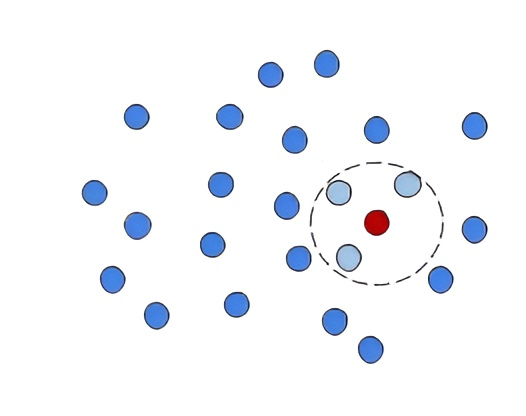
\includegraphics[width=0.5\columnwidth]{../img/related/knn.jpg}
		\caption{Brute-force retrieval of 3-Nearest Neighbors (light blue) for a query vector (red) from the dataset (blue)}        
		\label{fig:KNN_retrieval}
\end{figure}

To address this inefficiency, modern techniques focus on either reducing the dimensionality \(d\) through summarization or decreasing the number of comparisons by leveraging efficient indexing structures. These indexing structures prune unnecessary comparisons to \(V_Q\), thereby significantly improving performance. While some methods guarantee exact results, others aim for approximate answers—either with theoretical guarantees like \(\epsilon\)-approximations, or practical but non-guaranteed approaches, such as ng-approximation.

\noindent{\textbf{Summarization Techniques:}} Summarization techniques are fundamental to improving the efficiency of approximate similarity search by reducing the dimensionality of high-dimensional vectors, thus enabling faster search over large datasets. These methods attempt to transform or compress vectors into lower-dimensional representations while maintaining their key structural properties, speeding up the search while keeping accuracy loss to a minimum.

\begin{figure}[ht] 
\centering
		\captionsetup{justification=centering}
		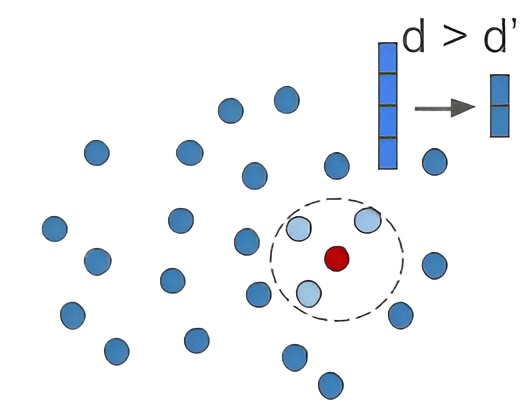
\includegraphics[width=0.5\columnwidth]{../img/related/sumb.jpg}
		\caption{Retrieval of 3-Nearest Neighbors (light blue) for a query vector (red) from the dataset (blue) summarized in lower dimensions}        
		\label{fig:sum_retrieval}
\end{figure}

For high-dimensional vectors, one of the most well-known summarization methods is \textit{Quantization}, which compresses continuous vector values into a finite set of codewords stored in a codebook. \textit{Product Quantization} (PQ)~\cite{jegou11} , along with optimized versions such as \textit{Optimized Product Quantization} (OPQ), divides the vector into subvectors, applies quantization to each, and forms the codebook by taking the Cartesian product of the subvector codebooks. This method strikes a balance between compression and search quality, enabling efficient storage and search in memory for large datasets, though it introduces some loss of accuracy due to compression.

For time-series data, several summarization techniques that are traditionally used have been adapted to high-dimensional vectors. \textit{Piecewise Aggregate Approximation} (PAA)~\cite{journal/kais/Keogh2001} and \textit{Adaptive Piecewise Constant Approximation} (APCA)~\cite{journal/acds/Chakrabarti2002} both segment vectors into either equal or variable-length portions, summarizing each segment by its mean. \textit{Extended APCA} (EAPCA)~\cite{conf/vldb/Wang2013} enhances this by including both the mean and standard deviation for each segment. Another approach, \textit{Symbolic Aggregate Approximation} (SAX)~\cite{conf/dmkd/LinKLC03}, transforms vectors using PAA and then assigns each segment a discrete symbol.

\textit{Random Projections} provide an alternative method for reducing dimensionality by projecting high-dimensional vectors into a lower-dimensional space through random matrices. According to the Johnson-Lindenstrauss lemma~\cite{conf/map/johnson84}, pairwise distances between vectors are approximately preserved in the lower-dimensional space, ensuring that search accuracy is maintained. The \textit{Karhunen-Lo\`{e}ve Transform (KLT)}~\cite{karhunen1947ueber,loeve1948functions} is another dimensionality reduction technique that decorrelates dimensions through linear transformation, followed by scalar quantization.

More recently, deep learning-based summarization techniques, like \textit{Deep Embedding Approximation} (DEA), have leveraged neural networks, such as SEAnet~\cite{seanetjournal}, to create data-driven summaries that adapt to the data distribution and enhance search performance.

\noindent{\textbf{Tree-based Indexes:}} Tree-based indexing structures organize data hierarchically to efficiently prune the search space. These structures have been a long-standing solution for exact vector search, especially for both data series and high-dimensional vectors~\cite{conf/sigmod/Guttman1984,conf/icmd/Beckmann1990,journal/edbt/Schafer2012,dstree,ulissejournal}. By partitioning the data into smaller regions, they reduce the search space and improve efficiency, with classical methods such as kd-trees and R-trees following predefined partitioning rules~\cite{flann,hdindex}.

\begin{figure}[ht] 
\centering
		\captionsetup{justification=centering}
		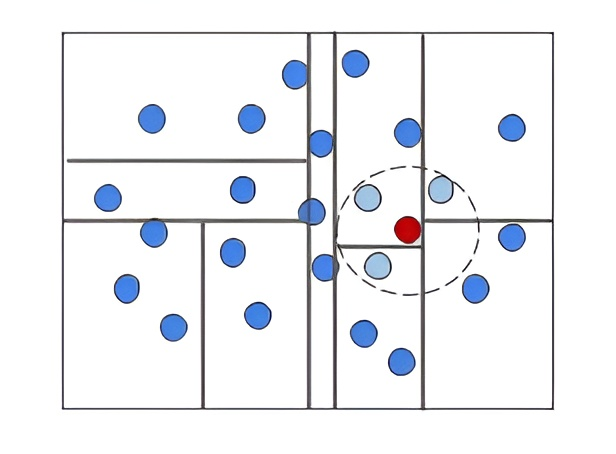
\includegraphics[width=0.5\columnwidth]{../img/related/treeb.jpg}
		\caption{Retrieval of 3-Nearest Neighbors (light blue) for a query vector (red) using a Tree-based index}        
		\label{fig:tree_retrieval}
\end{figure}

Tree-based methods for approximate similarity search have evolved to support both guaranteed and non-guaranteed searches (\textit{ng-approximate}). Exact methods use lower-bounding techniques to prune the search space without false negatives~\cite{conf/sigmod/Faloutsos1994}, whereas ng-approximate methods relax these guarantees to prioritize efficiency. For example, \textit{FLANN} constructs multiple randomized kd-trees and searches them in parallel, while \textit{HDIndex} segments the space into smaller regions, applying heuristics to speed up search~\cite{flann,hdindex}.

In ng-approximate search, tree-based methods often strike a balance between accuracy and efficiency by allowing users to specify parameters such as the number of leaves to visit or the search depth~\cite{hydra2,dumpy}. Some techniques apply dimensionality reduction before indexing~\cite{journal/kais/Camerra2014,journal/vldb/Zoumpatianos2016,dstree,ulisse,hercules}, while others index high-dimensional vectors directly~\cite{conf/vldb/Ciaccia1997}.

\noindent{\textbf{Hash-based Approaches:}} Hash-based methods, particularly those in the \textit{locality-sensitive hashing} (LSH) family~\cite{conf/stoc/indyk1998,lsh-survey}, are designed for \(\delta\)-\(\epsilon\)-approximate vector search. These methods use hash functions to map similar vectors into the same bucket with high probability, thus reducing the search space for high-dimensional vectors by clustering similar ones together.

\begin{figure}[ht] 
\centering
		\captionsetup{justification=centering}
		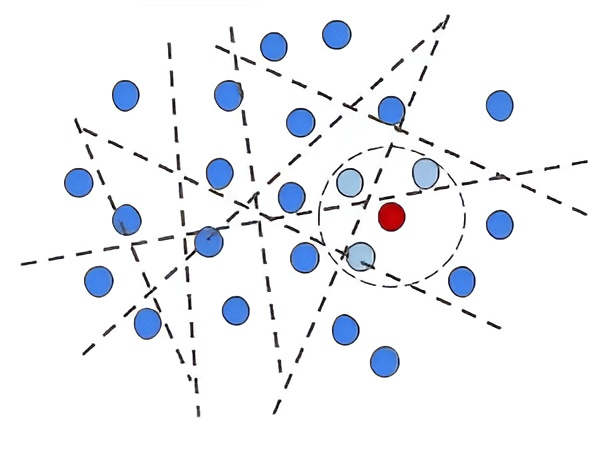
\includegraphics[width=0.5\columnwidth]{../img/related/hashb.jpg}
		\caption{Retrieval of 3-Nearest Neighbors (light blue) for a query vector (red) using Hash-based indexing}        
		\label{fig:hash_retrieval}
\end{figure}

Different variants of LSH have been proposed to optimize various aspects of search performance. \textit{Spherical Random Projection (SRS)}~\cite{srs} balances search efficiency with index size using random projections that maintain pairwise distances. \textit{Query-Aware Locality Sensitive Hashing (QALSH)}~\cite{qalsh} adjusts the hashing process to improve accuracy by incorporating the query vector into the hash function.

The trade-off between efficiency and accuracy in \(\delta\)-\(\epsilon\)-approximate searches can be fine-tuned by adjusting parameters such as the number of hash tables, the number of hash functions per table, and the number of random projections~\cite{qalsh,hydra2}. This flexibility makes hash-based methods an effective choice for fast search times with controllable approximation errors.

\noindent{\textbf{Graph-based Approaches:}} Graph-based methods support \textit{ng}-approximate vector search by organizing data into proximity graphs~\cite{gabriel69,toussaint02}. In such graphs, each vertex represents a data point, and edges are formed between vertices based on their proximity in the vector space, often determined by a distance measure like Euclidean distance~\cite{edelsbrunner87}. Graph traversal starts from a set of seed vertices, progressing in a best-first, greedy fashion until no better candidates are found~\cite{beamsearch}.

\begin{figure}[ht] 
\centering
		\captionsetup{justification=centering}
		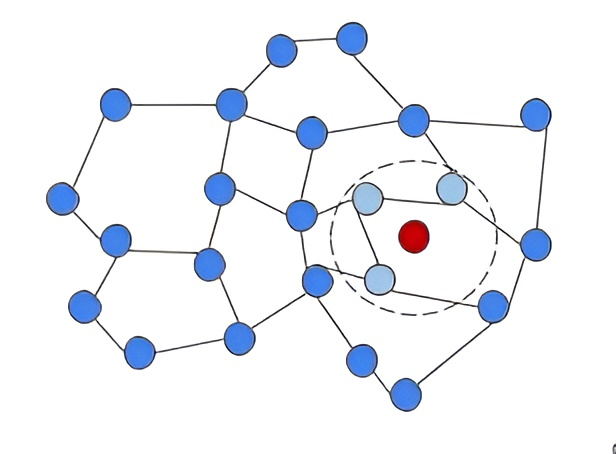
\includegraphics[width=0.5\columnwidth]{../img/related/graphb.jpg}
		\caption{Retrieval of 3-Nearest Neighbors (light blue) for a query vector (red) using Graph-based index structure}        
		\label{fig:graph_retrieval}
\end{figure}

State-of-the-art methods like \textit{KGraph}~\cite{kgraph}, \textit{HNSW}~\cite{hnsw}, \textit{NSG}~\cite{nsg}, \textit{Vamana}~\cite{vamana}, and \textit{ELPIS}~\cite{elpis} apply this general framework, but differ in how they construct the graph and choose initial entry points. These methods aim to strike a balance between connecting both short and long-range vertices while maintaining a sparse graph to minimize distance calculations, all while avoiding local minima.

The main challenge lies in managing this trade-off: too many edges complicate the routing process, while too few risk trapping the search in suboptimal regions of the graph. Modern graph-based methods focus on optimizing sparsity while maintaining robust connectivity, achieving high-speed, accurate search performance in large-scale vector datasets~\cite{hydra2,hnsw,nsg}.

\section{Summary of Approximate Search Methods}
\label{sec:summary_search_methods}

This section provides a summary of the key approximate similarity search methods, highlighting their primary strengths and weaknesses. Table~\ref{tab:methods_summary} presents an overview of the main characteristics, pros, and cons of each method.

\begin{table}[ht]
\centering
\begin{tabular}{|p{3cm}|p{4cm}|p{4cm}|p{4cm}|}
\hline
\textbf{Method} & \textbf{Description} & \textbf{Pros} & \textbf{Cons} \\ \hline
\textbf{Tree-based} & Organizes data in a hierarchical tree structure, enabling efficient pruning of the search space. & 
1. Low index construction time.
\newline 
2. Can support various search approaches.
& 
1. Lower search performance on difficult query workloads. \\ \hline

\textbf{Hash-based (LSH)} & Maps high-dimensional vectors into buckets using hash functions to group similar vectors. & 
1. Provides theoretical guarantees on query efficiency and accuracy. & 
1. Requires tuning multiple parameters (hash tables, hash functions). \newline 2. May reduce accuracy due to random hash assignments. \\ \hline

\textbf{Graph-based} & Constructs a proximity graph connecting vertices based on similarity, using greedy search to find neighbors. & 
1. Excellent empirical accuracy and efficiency.
& 
1. High index construction time and memory usage. \newline 2. Risk of getting stuck in local minima during search. \\ \hline
\end{tabular}
\caption{Summary of Approximate Search Methods: Pros and Cons}
\label{tab:methods_summary}
\end{table}

The major classes of approximate similarity search methods each present their own advantages and limitations. Tree-based methods provide hierarchical data organization, allowing for efficient pruning with relatively low index construction time, though they struggle with complex queries. Hash-based methods (LSH) group similar vectors into buckets, offering theoretical guarantees on performance, but require careful tuning and can suffer from reduced accuracy. Graph-based methods use proximity graphs to achieve high accuracy and efficient searching, but the high cost of building the index and the memory footprint are potential downsides.

\section{In-Memory vs Disk-Based Similarity Search}

Approximate similarity search algorithms can be broadly categorized into two approaches: \textit{in-memory} and \textit{disk-based} (or out-of-core). Both approaches aim to efficiently manage the retrieval of similar items from large-scale datasets but differ significantly in their handling of data storage and access.

\textbf{In-memory} approaches store all necessary data structures, such as proximity graphs or hash tables, in the main memory, enabling rapid access to data during query execution. These methods are highly efficient for query latency, as memory access times are orders of magnitude faster than disk operations. However, they are constrained by the machine's available memory, limiting their applicability to datasets that can fully reside within the main memory. In-memory methods are often the preferred choice for applications that require real-time or low-latency responses, such as recommendation systems or large-scale data retrieval tasks. Popular graph-based methods like HNSW~\cite{hnsw} and Vamana~\cite{vamana} have demonstrated excellent performance in in-memory settings but require significant memory resources during both graph construction and search.

\textbf{Disk-based} or \textit{out-of-core} approaches use the disk as an extension of the main memory, loading data segments into memory only as needed. This allows the algorithm to handle much larger datasets, often beyond the capacity of the machine’s RAM. Disk-based methods involve more complex data access patterns, which introduce significant I/O overhead, particularly when random disk accesses are required. To mitigate this, out-of-core algorithms often employ strategies that minimize random disk access by maximizing sequential I/O operations and improving data locality. For example, systems like DiskANN~\cite{vamana} and Hercules~\cite{hercules} provide disk-based solutions that can scale to extremely large datasets by efficiently managing memory and disk interactions, albeit at the cost of increased query latency.

Given the widespread use of large-scale datasets in modern similarity search applications, this thesis focuses on \textit{in-memory graph-based approaches}, which are particularly suitable for scenarios where fast query response times are critical, and the dataset can fit within available memory. While in-memory approaches offer significant advantages in terms of low latency and high query throughput, they are inherently limited by memory capacity, making them less practical for extremely large datasets that exceed memory limits. Nevertheless, for applications requiring high efficiency and manageable dataset sizes, in-memory graph-based methods strike a balance between query performance and accuracy. The following chapters will explore these techniques, presenting new optimizations aimed at improving their scalability and performance on large-scale data collections.

\section{Conclusion}

\noindent This chapter presented an overview of the main categories of approximate similarity search techniques, covering tree-based, hash-based, and graph-based methods. Each approach has distinct strengths and limitations in terms of performance, accuracy, and scalability, making them suitable for different scenarios and types of data. Tree-based methods are versatile, supporting multiple search strategies, but tend to underperform on complex or challenging workloads. Hash-based methods offer strong theoretical guarantees but require careful parameter tuning. In contrast, graph-based methods, though computationally more expensive to construct, have consistently shown superior empirical performance for large-scale datasets.

The following chapter will explore graph-based methods in greater detail, introducing a new taxonomy and key design paradigms that distinguish the various techniques. This will serve as a foundation for the development of novel methods aimed at further enhancing the efficiency of graph-based similarity search.
